\chapter{PRUEBAS Y RESULTADOS}
En esta fase del proyecto, se llevaron a cabo diversas pruebas para comprobar el correcto funcionamiento y verificar la calidad del intérprete, basándonos en los ocho puntos definidos por la norma ISO 25010. Para asegurar que el intérprete cumple con los estándares de calidad, se realizaron encuestas a los usuarios y pruebas directas al intérprete.

\section{Funcionalidad}
Esta prueba evalúa si el intérprete cumple con sus funciones básicas y requerimientos especificados.

Para esta prueba usamos una parte de la encuesta realizada a los usuarios que probaron el intérprete. Con esta verificamos si se encontraron errores durante la ejecución.
\begin{table}[!h]
  \begin{center}
    \begin{tabularx}{0.9\textwidth}{|X|X|}
      \hline
      \textbf{Pregunta} & \textbf{Descripción} \\
      \hline
      ¿Encontró algún error o problema técnico durante el uso del intérprete? & Esta pregunta identifica fallos funcionales. \\
      \hline
      Si respondió "Sí" en la pregunta anterior, por favor detalle el problema: & Los detalles aquí proporcionados serán utilizados para identificar problemas específicos y áreas que necesitan mejoras. \\
      \hline
    \end{tabularx}
  \end{center}
  \caption{Partes de la encuesta de funcionalidad}
  \centering Fuente: Elaboración propia
  \label{tab:funcionalidad}
\end{table}

Para esta prueba usamos una parte de la encuesta realizada a los usuarios que probaron el intérprete. Con esta verificamos si se encontraron errores durante la ejecución.

La Eficiencia en la Eliminación de Defectos (EED) es una medida utilizada en la gestión de la calidad para evaluar cuántos defectos se eliminan en relación con el esfuerzo total invertido en la detección y corrección de esos defectos. Se calcula utilizando la siguiente fórmula:
\begin{equation*}
  \begin{split}
    EED = \frac{(D - D_r)}{D} \times 100\%
  \end{split}
\end{equation*}

Donde:
\begin{equation*}
  \begin{split}
    D & \quad \textnormal{Es el número total de defectos antes de la corrección.}\\
    D_r & \quad \textnormal{Es el número de defectos restantes después de la corrección.}
  \end{split}
\end{equation*}

Antes de pasar a la etapa de pruebas con el software se encontraron los siguientes errores.

\begin{itemize}
  \item Error en la comparación de variables.
  \item Error en asignación de variables con ñ.
  \item Ejecución del bucle infinito en algunas ejecuciones de para (for).
  \item Error al cerrar una función.
  \item No se puede re-asignar una variable.
  \item No reconoce el salto de línea.
  \item Error al tener un si (if) dentro de un para (for).
  \item Error durante la instalación del intérprete.
  \item No se agrega al path de las variables de entorno.
\end{itemize}

Previamente se presentaron estos 9 errores.

Durante la recolección de datos, los usuarios reportaron este problema.
\begin{itemize}
  \item El poder instalar, porque se bloqueaba al descargar.
  \item No corre poniendo el comando dado en la terminal o tal vez no está muy  bien explicado.
\end{itemize}

De estos reportes, uno hace referencia a los errores previos y de funcionalidad.

Por lo tanto, tenemos que:
\begin{equation*}
  \begin{split}
    EED & = \frac{(9 - 1)}{9} \times 100\% \\
    EED & = 88.89 \%
  \end{split}
\end{equation*}

Por lo se deduce que se cuenta con una funcionalidad aceptable y también se debe trabajar en un error nuevo que se presentó, relacionado con la comprensión de la documentación.

\section{Fiabilidad}
Esta prueba evalúa la estabilidad y consistencia del intérprete bajo condiciones de uso normales.

Para esta prueba usamos una parte de la encuesta realizada a los usuarios que probaron el intérprete. Con esta calificamos la experiencia con el intérprete.
\begin{table}[!h]
  \begin{center}
    \begin{tabularx}{0.9\textwidth}{|X|X|}
      \hline
      \textbf{Pregunta} & \textbf{Descripción} \\
      \hline
      ¿Cuál fue su experiencia con el intérprete? & Permite evaluar la percepción general sobre la fiabilidad del intérprete. \\
      \hline
    \end{tabularx}
  \end{center}
  \caption{Partes de la encuesta, fiabilidad}
  \centering Fuente: Elaboración propia
  \label{tab:fiabilidad}
\end{table}

A continuación se muestra la escala de valores utilizada para evaluar la fiabilidad. Esta escala considera diferentes niveles, cada uno asociado con un valor específico y la cantidad correspondiente de casos evaluados.
\begin{table}[!h]
  \begin{center}
    \begin{tabularx}{0.9\textwidth}{|X|X|X|}
      \hline
      \textbf{Escala} & \textbf{Valor} & \textbf{Cantidad} \\
      \hline
      Muy buena & 5 & 15 \\
      \hline
      Buena & 4 & 25 \\
      \hline
      Regular & 3 & 12 \\
      \hline
      Mala & 2 & 1 \\
      \hline
      Muy mala & 1 & 0 \\
      \hline
    \end{tabularx}
  \end{center}
  \caption{Escala de valores para la fiabilidad}
  \centering Fuente: Elaboración propia
  \label{tab:fiabilidad-escala}
\end{table}

Realizando una media de los datos obtenidos tenemos:
\begin{equation*}
  \begin{split}
    \textnormal{Fiabilidad} & = \frac{\sum (\textnormal{valor} \times \textnormal{cantidad})}{5 \times \sum \textnormal{cantidad}} \times 100\% \\
    \textnormal{Fiabilidad} & = \frac{(5 \times 15 + 4 \times 25 + 3 \times 12 \times 2)}{5 \times 53} \times 100\% \\
    \textnormal{Fiabilidad} & = 80.38\%
  \end{split}
\end{equation*}

Por lo tanto, se puede concluir que la fiabilidad del intérprete es buena. Sin embargo, se debe trabajar en mejorar la percepción de los usuarios.

\section{Usabilidad}
Esta prueba evalúa qué tan fácil y agradable es para los usuarios interactuar con el intérprete.

Para esta prueba usamos una parte de la encuesta realizada a los usuarios que probaron el intérprete. Con esta calificamos el nivel de usabilidad que tiene el intérprete.
\begin{table}[!h]
  \begin{center}
    \begin{tabularx}{0.9\textwidth}{|X|X|}
      \hline
      \textbf{Pregunta} & \textbf{Descripción} \\
      \hline
      ¿Cómo calificaría la facilidad de uso del intérprete? & Se centra en la experiencia directa con la interfaz del intérprete. \\
      \hline
    \end{tabularx}
  \end{center}
  \caption{Partes de la encuesta, usabilidad}
  \centering Fuente: Elaboración propia
  \label{tab:usabilidad}
\end{table}

A continuación se muestra la escala de valores utilizada para evaluar la usabilidad. Esta escala considera diferentes niveles, cada uno asociado con un valor específico y la cantidad correspondiente de casos evaluados.

\begin{table}[!h]
  \begin{center}
    \begin{tabularx}{0.9\textwidth}{|X|X|X|}
      \hline
      \textbf{Escala} & \textbf{Valor} & \textbf{Cantidad} \\
      \hline
      Muy fácil & 5 & 14 \\
      \hline
      Fácil & 4 & 22 \\
      \hline
      Regular & 3 & 17 \\
      \hline
      Difícil & 2 & 0 \\
      \hline
      Muy difícil & 1 & 0 \\
      \hline
    \end{tabularx}
  \end{center}
  \caption{Escala de valores para la usabilidad}
  \centering Fuente: Elaboración propia
  \label{tab:usabilidad-escala}
\end{table}

Realizando una media de los datos obtenidos tenemos:
\begin{equation*}
  \begin{split}
    \textnormal{Usabilidad} & = \frac{\sum (\textnormal{valor} \times \textnormal{cantidad})}{5 \times \sum \textnormal{cantidad}} \times 100\% \\
    \textnormal{Usabilidad} & = \frac{(5 \times 14 + 4 \times 22 + 3 \times 17)}{5 \times 53} \times 100\% \\
    \textnormal{Usabilidad} & = 78.87\%
  \end{split}
\end{equation*}

Por lo tanto, se puede concluir que la usabilidad del intérprete es buena. Sin embargo, se debe trabajar en mejorar la percepción de los usuarios.

\section{Eficiencia}
Esta prueba analiza el rendimiento del intérprete, incluyendo velocidad y consumo de recursos.

Para esta prueba usamos una parte de la encuesta realizada a los usuarios que probaron el intérprete. Con esta calificamos el nivel de eficiencia que presenta el intérprete.
\begin{table}[!h]
  \begin{center}
    \begin{tabularx}{0.9\textwidth}{|X|X|}
      \hline
      \textbf{Pregunta} & \textbf{Descripción} \\
      \hline
      ¿Qué tan rápido y eficiente considera que es el intérprete en su ejecución? & Esta pregunta proporciona una evaluación subjetiva de la eficiencia del intérprete. \\
      \hline
    \end{tabularx}
  \end{center}
  \caption{Partes de la encuesta, eficiencia}
  \centering Fuente: Elaboración propia
  \label{tab:eficiencia}
\end{table}

A continuación se muestra la escala de valores utilizada para evaluar la eficiencia. Esta escala considera diferentes niveles, cada uno asociado con un valor específico y la cantidad correspondiente de casos evaluados.

\begin{table}[!h]
  \begin{center}
    \begin{tabularx}{0.9\textwidth}{|X|X|X|}
      \hline
      \textbf{Escala} & \textbf{Valor} & \textbf{Cantidad} \\
      \hline
      Muy rápido & 5 & 27 \\
      \hline
      Rápido & 4 & 24 \\
      \hline
      Regular & 3 & 2 \\
      \hline
      Lento & 2 & 0 \\
      \hline
      Muy lento & 1 & 0 \\
      \hline
    \end{tabularx}
  \end{center}
  \caption{Escala de valores para la eficiencia}
  \centering Fuente: Elaboración propia
  \label{tab:eficiencia-escala}
\end{table}

Realizando una media de los datos obtenidos tenemos:
\begin{equation*}
  \begin{split}
    \textnormal{Eficiencia} & = \frac{\sum (\textnormal{valor} \times \textnormal{cantidad})}{5 \times \sum \textnormal{cantidad}} \times 100\% \\
    \textnormal{Eficiencia} & = \frac{(5 \times 27 + 4 \times 24 + 3 \times 2)}{5 \times 53} \times 100\% \\
    \textnormal{Eficiencia} & = 89.43\%
  \end{split}
\end{equation*}

Por lo tanto, se puede concluir que la eficiencia del intérprete es muy buena. Sin embargo, se debe trabajar en mejorar la percepción de los usuarios.

\section{Mantenibilidad}
Para asegurar la mantenibilidad de nuestro proyecto según la norma ISO/IEC 25010, hemos implementado una documentación exhaustiva y una estructura de código modular y limpia. La documentación incluye guías de usuario, manuales técnicos y procedimientos de instalación que facilitan la comprensión y contribución al proyecto. Además, el código está diseñado con nombres descriptivos y comentarios claros, siguiendo las mejores prácticas de programación. Hemos establecido una cobertura de pruebas robusta con pruebas unitarias, de integración y de sistema, y utilizamos un sistema de control de versiones con Git, asegurando un flujo de trabajo eficiente con commits documentados y ramas claramente definidas.

\section{Portabilidad}
El intérprete puede ser instalado y utilizado de manera efectiva en diferentes sistemas operativos como Linux y Windows. Esta característica se logra mediante el uso de tecnologías y prácticas que aseguran su compatibilidad y rendimiento óptimo en ambas plataformas sin necesidad de modificaciones adicionales por parte del usuario.

\section{Seguridad}
Para garantizar la integridad del código, se emplearon las herramientas proporcionadas por GitHub:
\begin{itemize}
  \item \textbf{Gestión de Accesos y Colaboradores} \\
  Se configuraron cuidadosamente los permisos de acceso al repositorio.
  \item \textbf{Política de Revisión de Código} \\
  Se ha definido una política clara de revisión de código que asegura que todas las contribuciones enviadas mediante pull requests serán cuidadosamente revisadas antes de su integración en la rama principal del proyecto.
  \item \textbf{Gestión de Issues y Pull Requests} \\
  Se ha establecido un sistema de seguimiento de problemas y solicitudes de cambios que permite a los colaboradores reportar errores y proponer mejoras de manera segura y eficiente.
\end{itemize}

\begin{figure}[!h]
  \centering
  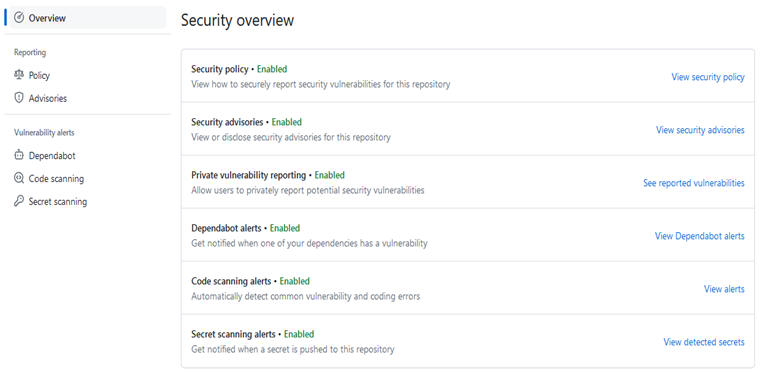
\includegraphics[width=0.8\textwidth]{images/seguridad.png}
  \caption{Seguridad}
  \centering Fuente: Elaboración propia
  \label{fig:seguridad}
\end{figure}

\section{Compatibilidad}
Se garantizó la compatibilidad del intérprete desarrollado mediante la implementación de la capacidad para ejecutar archivos exclusivos con extensión “.inf”. Estos archivos a su vez tienen una estructura clara, que se detalla en la documentación, si se sigue la estructura planteada y se le asigna la extensión adecuada, entonces se garantiza que el archivo es portable en cualquier sistema operativo que se encuentre instalado.

\section{Prueba de hipótesis}
\begin{itemize}
  \item \textbf{Variable Dependiente (VD):} La percepción media de los usuarios sobre la fiabilidad, usabilidad y eficiencia del intérprete.
  \item \textbf{Variable Independiente (VI):} El nivel aceptable $(3)$.
  \item \textbf{H0 (Hipótesis nula):} La percepción media de los usuarios sobre la fiabilidad, usabilidad y eficiencia del intérprete es igual o menor a un nivel aceptable $(3)$.
  \item \textbf{H1 (Hipótesis alternativa):} La percepción media de los usuarios sobre la fiabilidad, usabilidad y eficiencia del intérprete es mayor que un nivel aceptable $(>3)$.
\end{itemize}

\subsection{Prueba t de student}
La prueba t de una sola muestra compara la media de un solo grupo con un valor de referencia conocido.

\begin{center}
  \begin{longtable}{|l|l|l|l|}
    \hline
    & \textbf{Fiabilidad} & \textbf{Usabilidad} & \textbf{Eficiencia} \\
    \hline
    \endfirsthead
    \hline
    \endhead
    \endfoot
    \hline
    1 & 3 & 3 & 5 \\
    \hline
    2 & 3 & 3 & 3 \\
    \hline
    3 & 3 & 5 & 5 \\
    \hline
    4 & 4 & 3 & 5 \\
    \hline
    5 & 3 & 3 & 5 \\
    \hline
    6 & 3 & 3 & 5 \\
    \hline
    7 & 3 & 2 & 3 \\
    \hline
    8 & 3 & 3 & 4 \\
    \hline
    9 & 3 & 4 & 5 \\
    \hline
    10 & 3 & 4 & 5 \\
    \hline
    11 & 3 & 4 & 5 \\
    \hline
    12 & 3 & 3 & 5 \\
    \hline
    13 & 3 & 3 & 5 \\
    \hline
    14 & 4 & 4 & 4 \\
    \hline
    15 & 4 & 4 & 5 \\
    \hline
    16 & 4 & 4 & 4 \\
    \hline
    17 & 3 & 4 & 3 \\
    \hline
    18 & 4 & 3 & 5 \\
    \hline
    19 & 3 & 4 & 5 \\
    \hline
    20 & 3 & 3 & 4 \\
    \hline
    21 & 3 & 3 & 5 \\
    \hline
    22 & 3 & 3 & 4 \\
    \hline
    23 & 4 & 4 & 4 \\
    \hline
    24 & 5 & 5 & 5 \\
    \hline
    25 & 5 & 5 & 4 \\
    \hline
    26 & 5 & 5 & 5 \\
    \hline
    27 & 4 & 4 & 4 \\
    \hline
    28 & 4 & 4 & 4 \\
    \hline
    29 & 5 & 5 & 5 \\
    \hline
    30 & 5 & 5 & 5 \\
    \hline
    31 & 5 & 5 & 5 \\
    \hline
    32 & 5 & 5 & 5 \\
    \hline
    33 & 5 & 5 & 5 \\
    \hline
    34 & 5 & 5 & 5 \\
    \hline
    35 & 5 & 5 & 5 \\
    \hline
    36 & 4 & 4 & 4 \\
    \hline
    37 & 4 & 4 & 4 \\
    \hline
    38 & 5 & 5 & 5 \\
    \hline
    39 & 5 & 5 & 5 \\
    \hline
    40 & 4 & 4 & 4 \\
    \hline
    41 & 4 & 4 & 4 \\
    \hline
    42 & 4 & 4 & 4 \\
    \hline
    43 & 5 & 5 & 5 \\
    \hline
    44 & 4 & 4 & 4 \\
    \hline
    45 & 4 & 4 & 4 \\
    \hline
    46 & 4 & 4 & 4 \\
    \hline
    47 & 4 & 4 & 4 \\
    \hline
    48 & 4 & 4 & 4 \\
    \hline
    49 & 4 & 4 & 4 \\
    \hline
    50 & 4 & 4 & 4 \\
    \hline
    51 & 4 & 4 & 4 \\
    \hline
    52 & 4 & 4 & 4 \\
    \hline
    53 & 5 & 5 & 5 \\
    \hline
    \caption{Resultado en la percepción de los usuarios}
  \end{longtable}
  \vspace*{-2.5em}
  \centering Fuente: Elaboración propia
\end{center}

Calcular la media global.
\begin{equation*}
  \begin{split}
    \overline{X} & = \frac{\sum_{i=1}^{n} x_i}{n} \\
    \overline{X} & = \frac{658}{159} \\
    \overline{X} & = 4.138
  \end{split}
\end{equation*}

Calcular las medias de cada grupo.
\begin{equation*}
  \begin{split}
    \overline{X}_j & = \frac{\sum_{i=1}^{n} x_{ij}}{n}
  \end{split}
\end{equation*}

Fiabilidad:
\begin{equation*}
  \begin{split}
    \overline{X}_{fiabilidad} & = \frac{209}{53} \\
    \overline{X}_{fiabilidad} & = 3.943
  \end{split}
\end{equation*}

Usabilidad:
\begin{equation*}
  \begin{split}
    \overline{X}_{usabilidad} & = \frac{213}{40} \\
    \overline{X}_{usabilidad} & = 4.019
  \end{split}
\end{equation*}

Eficiencia:
\begin{equation*}
  \begin{split}
    \overline{X}_{eficiencia} & = \frac{236}{66} \\
    \overline{X}_{eficiencia} & = 4.453
  \end{split}
\end{equation*}

Grados de libertad $(df)$.
\begin{equation*}
  \begin{split}
    df & = n - 1 \\
    df & = 53 - 1 \\
    df & = 52
  \end{split}
\end{equation*}

Desviación estándar muestral.

Fiabilidad:
\begin{equation*}
  \begin{split}
    S_{fiabilidad} & = \sqrt{\frac{\sum_{i=1}^{n} (x_{i} - \overline{X}_{fiabilidad})^2}{n - 1}} \\
    S_{fiabilidad} & = \sqrt{\frac{30.830}{52}} \\
    S_{fiabilidad} & = 0.770
  \end{split}
\end{equation*}

Usabilidad:
\begin{equation*}
  \begin{split}
    S_{usabilidad} & = \sqrt{\frac{\sum_{i=1}^{n} (x_{i} - \overline{X}_{usabilidad})^2}{n - 1}} \\
    S_{usabilidad} & = \sqrt{\frac{30.981}{52}} \\
    S_{usabilidad} & = 0.772
  \end{split}
\end{equation*}

Eficiencia:
\begin{equation*}
  \begin{split}
    S_{eficiencia} & = \sqrt{\frac{\sum_{i=1}^{n} (x_{i} - \overline{X}_{eficiencia})^2}{n - 1}} \\
    S_{eficiencia} & = \sqrt{\frac{19.132}{52}} \\
    S_{eficiencia} & = 0.607
  \end{split}
\end{equation*}

Estadístico t.
\begin{equation*}
  \begin{split}
    t & = \frac{\overline{X} - \mu_0}{\frac{S}{\sqrt{n}}} \\
  \end{split}
\end{equation*}

Fiabilidad:
\begin{equation*}
  \begin{split}
    t_{fiabilidad} & = \frac{3.943 - 3}{\frac{0.770}{\sqrt{53}}} \\
    t_{fiabilidad} & = 8.920
  \end{split}
\end{equation*}

Usabilidad:
\begin{equation*}
  \begin{split}
    t_{usabilidad} & = \frac{4.019 - 3}{\frac{0.772}{\sqrt{40}}} \\
    t_{usabilidad} & = 9.610
  \end{split}
\end{equation*}

Eficiencia:
\begin{equation*}
  \begin{split}
    t_{eficiencia} & = \frac{4.453 - 3}{\frac{0.607}{\sqrt{66}}} \\
    t_{eficiencia} & = 17.437
  \end{split}
\end{equation*}

Valor crítico p.

Fiabilidad:
\begin{equation*}
  \begin{split}
    p_{fiabilidad} & = (t=8.920, df=52) \\
    p_{fiabilidad} & = 2.311 \times 10^{-12}
  \end{split}
\end{equation*}

Usabilidad:
\begin{equation*}
  \begin{split}
    p_{usabilidad} & = (t=9.610, df=39) \\
    p_{usabilidad} & = 2.020 \times 10^{-13}
  \end{split}
\end{equation*}

Eficiencia:
\begin{equation*}
  \begin{split}
    p_{eficiencia} & = (t=17.437, df=65) \\
    p_{eficiencia} & = 1.123 \times 10^{-23}
  \end{split}
\end{equation*}

El valor $p$ es extremadamente bajo en todos los casos (menor que cualquier nivel común de significancia, como $0.05, 0.01 o 0.001$), lo que sugiere que se rechaza la hipótesis nula en cada caso y aceptamos la hipótesis alternativa. 

Por lo tanto, podemos concluir que la percepción media de los usuarios sobre la fiabilidad, usabilidad y eficiencia del intérprete es mayor que un nivel aceptable $(>3)$.
